% \documentclass[table]{beamer}
\documentclass[table,handout]{beamer}
\setbeameroption{show notes}
% \setbeameroption{hide notes}
% \setbeameroption{show only notes}
\usepackage{varwidth}

\newif\ifhide
\newif\ifpost
\newif\ifhideclicker

% \hidetrue
% \hideclickertrue
% \posttrue

\newcommand{\whiteout}[1]{\textcolor{white}{#1}}
% \newcommand{\whiteoutbox}[1]{\fcolorbox{white}{white}{\parbox{\dimexpr \linewidth-2\fboxsep-2\fboxrule}{\whiteout{#1}}}}
% \newcommand{\notebox}[1]{\fcolorbox{blue}{white}{\parbox{\dimexpr \linewidth-2\fboxsep-2\fboxrule}{#1}}}
\newcommand{\whiteoutbox}[1]{\fcolorbox{white}{white}{\parbox{\linewidth}{\whiteout{#1}}}}
\newcommand{\notebox}[1]{\fcolorbox{blue}{white}{\parbox{\linewidth}{#1}}}
\newcommand{\blankbox}[1]{\phantom{\varwidth{\linewidth}\whiteoutbox{#1}\endvarwidth}}
\newcommand{\blank}[1]{\phantom{\varwidth{\linewidth}#1\endvarwidth}}

\ifhide%
    \newcommand{\hmask}[1]{\blank{#1}}%
\else%
    \newcommand{\hmask}[1]{#1}%
\fi

\ifhide%
    \newcommand{\wout}[1]{\whiteout{#1}}%
\else%
    \newcommand{\wout}[1]{#1}%
\fi

\ifhide%
    \newcommand{\hignore}[1]{}%
\else%
    \newcommand{\hignore}[1]{#1}%
\fi

\ifpost%
    \newcommand{\nopost}[1]{}%
\else%
    \newcommand{\nopost}[1]{#1}%
\fi

\ifhideclicker%
    \newcommand{\clickerslide}[1]{\stepcounter{clickerQuestionCounter}%
        \begin{frame}[t]
            \textcolor{blue}{Q \arabic{clickerQuestionCounter}:}
        \end{frame}}
\else%
    \newcommand{\clickerslide}[1]{#1}%
\fi

\ifhide%
    \newcommand{\hidebox}[1]{\blank{#1}}%
\else%
    \newcommand{\hidebox}[1]{\notebox{#1}}%
\fi

\ifhide%
    \newcommand{\wbox}[1]{\whiteoutbox{#1}}%
\else%
    \newcommand{\wbox}[1]{\notebox{#1}}%
\fi

\ifhide%
    \newcommand{\nbox}[1]{\blankbox{#1}}%
\else%
    \newcommand{\nbox}[1]{\notebox{#1}}%
\fi

\ifhideclicker%
    \newcommand{\clickeranswer}[1]{#1}%
\else%
    \ifhide%
        \newcommand{\clickeranswer}[1]{#1}%
    \else%
        \newcommand{\clickeranswer}[1]{\textbf{\textcolor{blue}{#1}}}%
    \fi
\fi

\usepackage{beamerthemesplit}
% \usetheme{boxes}
\usetheme{Malmoe}
\usecolortheme{seahorse}
% \usecolortheme{seagull}
\usepackage{ifthen}
\usepackage{xspace}
\usepackage{multirow}
\usepackage{multicol}
\usepackage{booktabs}
\usepackage{xcolor}
\usepackage{wasysym}
\usepackage{comment}
\usepackage{hyperref}
\hypersetup{pdfborder={0 0 0}, colorlinks=true, urlcolor=blue, linkcolor=blue, citecolor=blue}
\usepackage{changepage}
\usepackage[compatibility=false]{caption}
\captionsetup[figure]{font=scriptsize, labelformat=empty, textformat=simple, justification=centering, skip=2pt}
\usepackage{tikz}
\usetikzlibrary{trees,calc,backgrounds}

\usepackage[bibstyle=joaks-slides,maxcitenames=3,mincitenames=1,backend=biber]{biblatex}

\newrobustcmd*{\shortfullcite}{\AtNextCite{\renewbibmacro{title}{}\renewbibmacro{in:}{}\renewbibmacro{number}{}}\fullcite}

\newrobustcmd*{\footlessfullcite}{\AtNextCite{\renewbibmacro{title}{}\renewbibmacro{in:}{}}\footfullcite}

% Make all footnotes smaller
% \renewcommand{\footnotesize}{\scriptsize}

\definecolor{myGray}{gray}{0.9}
\colorlet{rowred}{red!30!white}

\setbeamertemplate{blocks}[rounded][shadow=true]

\setbeamercolor{defaultcolor}{bg=structure!30!normal text.bg,fg=black}
\setbeamercolor{block body}{bg=structure!30!normal text.bg,fg=black}
\setbeamercolor{block title}{bg=structure!50!normal text.bg,fg=black}

\newenvironment<>{varblock}[2][\textwidth]{%
  \setlength{\textwidth}{#1}
  \begin{actionenv}#3%
    \def\insertblocktitle{#2}%
    \par%
    \usebeamertemplate{block begin}}
  {\par%
    \usebeamertemplate{block end}%
  \end{actionenv}}

\newenvironment{displaybox}[1][\textwidth]
{
    \centerline\bgroup\hfill
    \begin{beamerboxesrounded}[lower=defaultcolor,shadow=true,width=#1]{}
}
{
    \end{beamerboxesrounded}\hfill\egroup
}

\newenvironment{onlinebox}[1][4cm]
{
    \newbox\mybox
    \newdimen\myboxht
    \setbox\mybox\hbox\bgroup%
        \begin{beamerboxesrounded}[lower=defaultcolor,shadow=true,width=#1]{}
    \centering
}
{
    \end{beamerboxesrounded}\egroup
    \myboxht\ht\mybox
    \raisebox{-0.25\myboxht}{\usebox\mybox}\hspace{2pt}
}

\newenvironment{mydescription}{
    \begin{description}
        \setlength{\leftskip}{-1.5cm}}
    {\end{description}}

\newenvironment{myitemize}{
    \begin{itemize}
        \setlength{\leftskip}{-.3cm}}
    {\end{itemize}}

% footnote without a marker
\newcommand\barefootnote[1]{%
  \begingroup
  \renewcommand\thefootnote{}\footnote{#1}%
  \addtocounter{footnote}{-1}%
  \endgroup
}

% define formatting for footer
\newcommand{\myfootline}{%
    {\it
    \insertshorttitle
    \hspace*{\fill} 
    \insertshortauthor, \insertshortinstitute
    % \ifx\insertsubtitle\@empty\else, \insertshortsubtitle\fi
    \hspace*{\fill}
    \insertframenumber/\inserttotalframenumber}}

% set up footer
\setbeamertemplate{footline}{%
    \usebeamerfont{structure}
    \begin{beamercolorbox}[wd=\paperwidth,ht=2.25ex,dp=1ex]{frametitle}%
        % \Tiny\hspace*{4mm}\myfootline\hspace{4mm}
        \tiny\hspace*{4mm}\myfootline\hspace{4mm}
    \end{beamercolorbox}}

% remove navigation bar
\beamertemplatenavigationsymbolsempty

\makeatletter
    \newenvironment{noheadline}{
        \setbeamertemplate{headline}[default]
        \def\beamer@entrycode{\vspace*{-\headheight}}
    }{}
\makeatother

\newcounter{clickerQuestionCounter}
\ifhideclicker%
\newenvironment{clickerquestion}
{ \stepcounter{clickerQuestionCounter}
  \begin{enumerate}[Q \arabic{clickerQuestionCounter}:]\color{white} }
{ \end{enumerate} }
\else%
\newenvironment{clickerquestion}
{ \stepcounter{clickerQuestionCounter}
  \begin{enumerate}[Q \arabic{clickerQuestionCounter}:] }
{ \end{enumerate} }
\fi

\ifhideclicker%
\newenvironment{clickeroptions}
{ \begin{enumerate}[\begingroup\color{white} 1)\endgroup]\color{white} }
{ \end{enumerate} }
\else%
\newenvironment{clickeroptions}
{ \begin{enumerate}[\begingroup\color{red} 1)\endgroup] }
{ \end{enumerate} }
\fi


\tikzstyle{centered} = [align=center, text centered, font=\sffamily\bfseries]
\tikzstyle{skip} = [centered, inner sep=0pt, fill]
\tikzstyle{empty} = [centered, inner sep=0pt]
\tikzstyle{inode} = [centered, circle, minimum width=4pt, fill=black, inner sep=0pt]
\tikzstyle{tnode} = [centered, circle, inner sep=1pt]
\tikzset{
  % edge styles
  level distance=10mm,
  mate/.style={edge from parent/.style={draw,distance=3pt}},
  mleft/.style={grow=left, level distance=10mm, edge from parent path={(\tikzparentnode.west)--(\tikzchildnode.east)}},
  mright/.style={grow=right, level distance=10mm, edge from parent path={(\tikzparentnode.east)--(\tikzchildnode.west)}},
  % node styles
  male/.style={rectangle,minimum size=4mm,fill=gray!80},
  female/.style={circle,minimum size=4mm,fill=gray!80},
  amale/.style={male,fill=red},
  afemale/.style={female,fill=red},
}

\newcommand{\highlight}[1]{\textcolor{violet}{\textit{\textbf{#1}}}}
\newcommand{\super}[1]{\ensuremath{^{\textrm{\sffamily #1}}}}
\newcommand{\sub}[1]{\ensuremath{_{\textrm{\sffamily #1}}}}
\newcommand{\dC}{\ensuremath{^\circ{\textrm{C}}}}
\newcommand{\tb}{\hspace{2em}}
\providecommand{\e}[1]{\ensuremath{\times 10^{#1}}}
\newcommand{\myHangIndent}{\hangindent=5mm}

\newcommand{\spp}[1]{\textit{#1}}

\newcommand\mybullet{\leavevmode%
\usebeamertemplate{itemize item}\hspace{.5em}}

\makeatletter
\newcommand*{\rom}[1]{\expandafter\@slowromancap\romannumeral #1@}
\makeatother

\newcommand{\blankslide}{{\setbeamercolor{background canvas}{bg=black}
\setbeamercolor{whitetext}{fg=white}
\begin{frame}<handout:0>[plain]
\end{frame}}}

\newcommand{\whiteslide}{
\begin{frame}<handout:0>[plain]
\end{frame}}

\newcommand{\f}[1]{\ensuremath{F_{#1}}}
\newcommand{\x}[1]{X\ensuremath{^{#1}}}
\newcommand{\y}[1]{Y\ensuremath{^{#1}}}

% Population growth macros
\newcommand{\popsize}[1]{\ensuremath{N_{#1}}}
\newcommand{\popgrowthratediscrete}[1]{\ensuremath{\lambda_{#1}}}
\newcommand{\popgrowthrate}[1]{\ensuremath{r_{#1}}}
\newcommand{\ptime}{\ensuremath{t}\xspace}

\tikzset{hide on/.code={\only<#1>{\color{white}}}}
\tikzset{
    invisible/.style={opacity=0},
    visible on/.style={alt={#1{}{invisible}}},
    alt/.code args={<#1>#2#3}{%
        \alt<#1>{\pgfkeysalso{#2}}{\pgfkeysalso{#3}}
        % \pgfkeysalso doesn't change the path
    },
}

\bibliography{../bib/references}
\author[J.\ Oaks]{
    %Jamie R.\ Oaks\inst{1}
    Jamie R.\ Oaks
}
\institute[BIOL 180]{
    \inst{}%
        BIOL 180: Introductory Biology
}



\title[Chromosome theory of inheritance]{Chromosome theory of inheritance}
% \date{\today}
\date{April 8, 2015}

\begin{document}

\begin{noheadline}
\maketitle
\end{noheadline}

\nopost{
\begin{noheadline}
\begin{frame}[c]
    \vspace{-6mm}
    \begin{center} 
        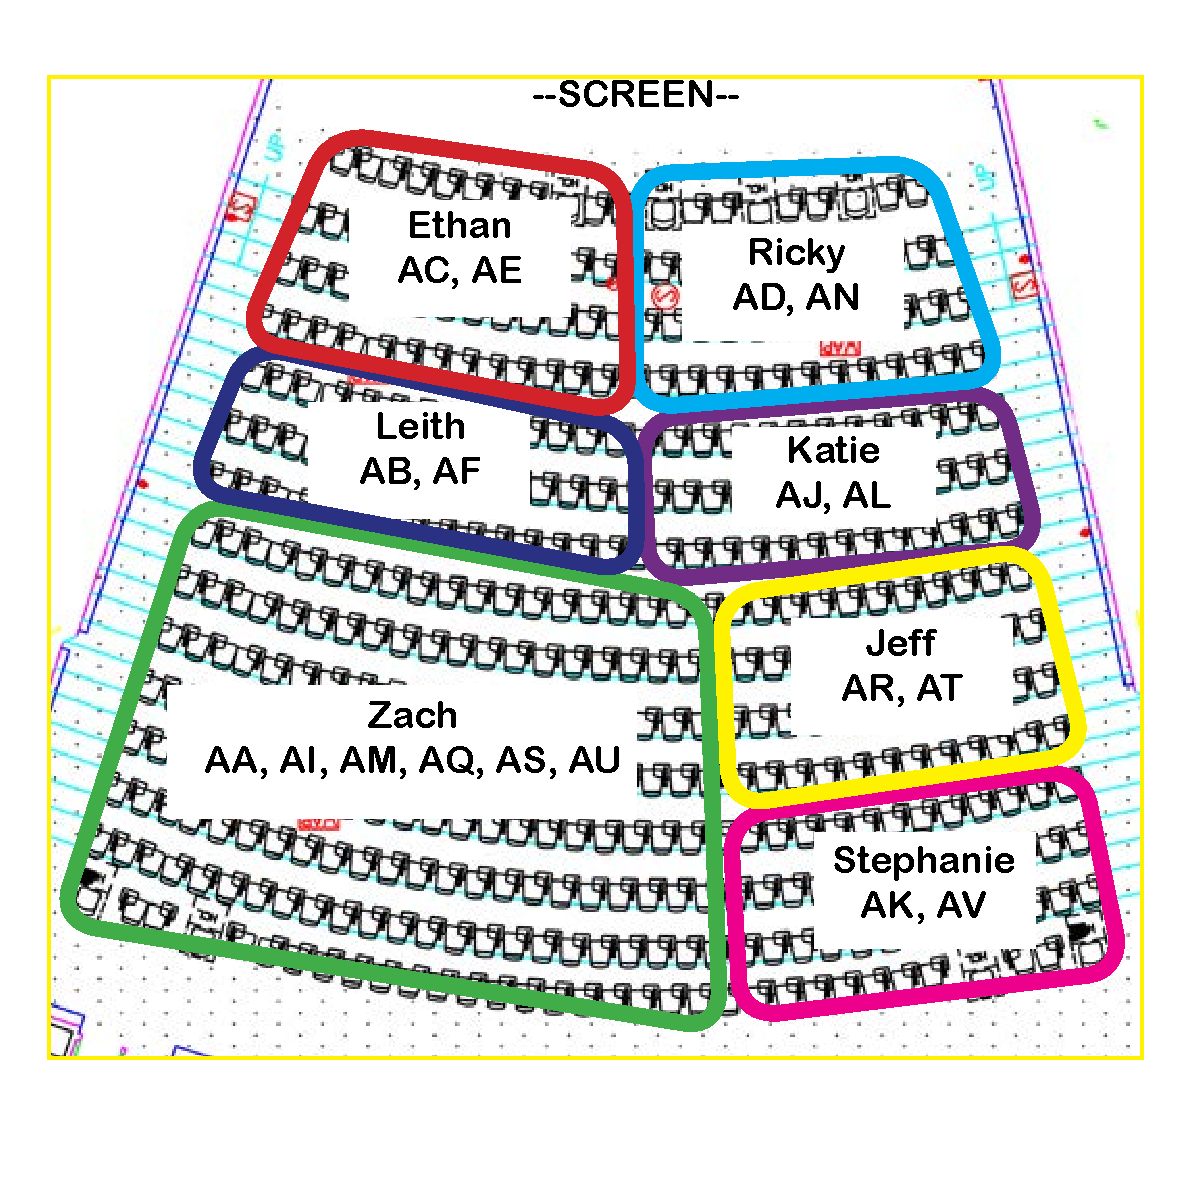
\includegraphics[height=1.3\textheight]{../images/seating-chart.pdf}
    \end{center}
\end{frame}
\end{noheadline}
}

\begin{noheadline}
\begin{frame}
\frametitle{Today's issues:}
What is the physical basis of Mendel's rules? \\
\vspace{5mm}
\tableofcontents[subsectionstyle=hide]
\end{frame}
\end{noheadline}

% \begin{noheadline}
% \begin{frame}
% \frametitle{Today's issues:}
% % \tableofcontents[subsectionstyle=hide]
% \begin{enumerate}
%     \item How are alleles from different genes transmitted to offspring
%         (together, or independently of each other?
%     \item What is the physical basis of Mendel's rules?
%         \begin{enumerate}
%             \item Mitosis: How cells divide during asexual reproduction and
%                 during growth
%             \item Meiosis: How cells divide prior to formation of eggs and
%                 sperm (sexual reproduction)
%         \end{enumerate}
% \end{enumerate}
% \end{frame}
% \end{noheadline}
\section{Pattern and process components of chromosome theory}

\clickerslide{
\begin{frame}
    \begin{clickerquestion}
        \item What event makes meiosis produce haploid daughter cells instead
            of diploid daughter cells (like mitosis)?
        \begin{clickeroptions}
            \item Chromosomes replicate prior to meiosis I, but not prior to
                meiosis II.
            \item Meiosis II and mitosis are identical, except that cells are
                haploid in meiosis II 
            \item Homologs go to the metaphase plate independently of each
                other.
            \item \clickeranswer{Homologs synapse and to to the metaphase plate
                    together.}
        \end{clickeroptions}
    \end{clickerquestion}
\end{frame}
}

\begin{frame}
    \frametitle{The chromosome theory of inheritance}
    \begin{description}
        \item[Pattern:] \nbox{``Mendel's rules''; Alleles of the same gene
                separate (segregation), and alleles of different genes separate
                independently (independent assortment)}
        \item[Process:] \nbox{Genes are on chromosomes that undergo
                \highlight{meiosis}}
    \end{description}
\end{frame}


\begin{frame}[t]
    \begin{adjustwidth}{-2em}{-2em}
    \vspace{-4mm}
    Proposition \#1: The principle of segregation results from the separation
    of homologous chromosomes at meiosis I. \\

    \vspace{3mm}
    Draw this for an individual with the genotype $Pp$ (draw replicated
    chromosomes and put alleles on them; what do they do during meiosis I?) \\

    \nbox{Should draw one homolog (two sister chromatids) with $P$ labeled, and
        the other homolog (sister chromatids) with $p$ labeled; draw them
        coming together (synapsing) and separating to different daughter cells}
    
    \end{adjustwidth}

    \note[item]{TAs may need to help with this}
\end{frame}

\begin{frame}[t]
    \begin{adjustwidth}{-2em}{-2em}
    \vspace{-4mm}
    Proposition \#2: The principle of independent assortment occurs because
    maternal and paternal homologs of different chromosomes line up
    independently of one another at metaphase of meiosis I \\

    \vspace{3mm}
    Draw this for an individual with the genotype $PpTt$ (draw replicated
    chromosomes and put alleles on them; what do they do during meiosis I?) \\

    \nbox{Should draw 2 pairs of homologs (a total of 4 replicated chromosomes)
        that synapse (2 synapsing pairs), line up randomly of one another, and
        pull apart (e.g., whether $P$ and $T$, or $P$ and $t$ end up on the
        same size is random)}

    \vspace{0.42\textheight}
    What are the gamete genotypes? \hmask{\highlight{\small $\frac{1}{4}PT, \frac{1}{4}Pt, \frac{1}{4}pT, \frac{1}{4}pt$}}

    \end{adjustwidth}

    \note[item]{TAs may need to help with this}
\end{frame}

\clickerslide{
\begin{frame}
    \begin{clickerquestion}
        \item  Which genes \textbf{violate} the principle of independent
            assortment?
        \begin{clickeroptions}
            \item Genes that are found on different chromosomes (if no crossing
                over occurs between them).
            \item \clickeranswer{Genes that are found on the same chromosomes
                    (if no crossing over occurs between them).}
            \item  Genes involved in ``discrete'' traits---like the 7 pea
                traits that Mendel analyzed
            \item Genes involved in ``continuous'' traits---like height in
                humans.
        \end{clickeroptions}
    \end{clickerquestion}
\end{frame}
}

\begin{frame}[plain]
    \note[item]{Draw the answer to the clicker question}
\end{frame}


\section{Testing the chromosome theory}

\begin{frame}
    \frametitle{What predictions does the chromosome theory make?}
    \begin{adjustwidth}{-2em}{-2em}
    If genes are found on chromosomes, then we should be able to determine the
    locations of specific genes (associate specific genes with specific
    chromosomes).

    \begin{columns}
        
        \column{0.55\linewidth}
        \begin{itemize}
            \item<2-> Fruit flies as model organism
            \item<3-> Discovery of white-eye mutants
            \item<4-> What's a mutant? \uncover<4->{\highlight{Novel
                        phenotype} (for now)}
        \end{itemize}

        \column{0.45\linewidth}
        \uncover<3->{
            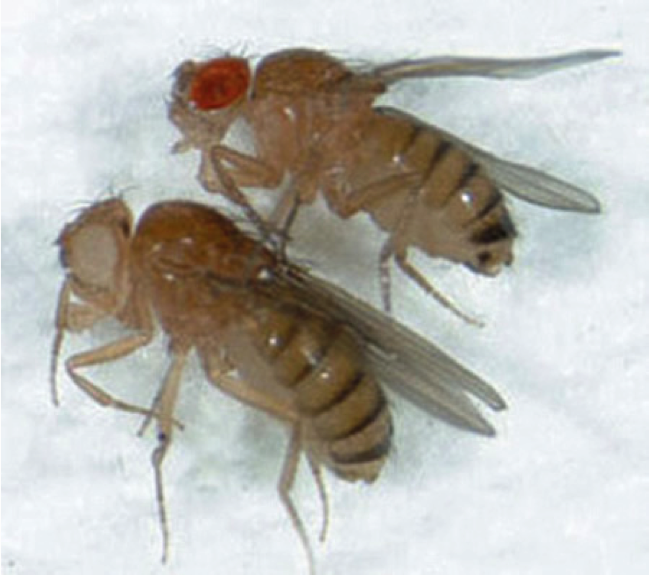
\includegraphics[width=\textwidth]{../images/drosophila-white-eye.png}
        }

    \end{columns}
    \end{adjustwidth}

    \note[item]{Undergrads working in Thomas Hunt Morgan's lab on fruit fly
        genetics found a white-eyed mutant}
    \note[item]{Started doing crosses to try to understand novel phenotype}
\end{frame}

\begin{frame}
    \frametitle{Crosses with white-eye mutant give weird results\ldots}
    \begin{itemize}[<+->]
        \item \textbf{Cross 1:} Red-eyed \female $\times$ white-eyed \male
            \begin{itemize}
                \item All \f{1}s have red eyes
            \end{itemize}

            \vspace{1cm}
        \item \textbf{Cross 2:} Let \f{1} males and females breed
            \begin{itemize}
                \item In \f{2}s, red-eyed to white-eyed phenotype ratio is 3:1

                \item What hypothesis would explain these data? \nbox{Red-eye
                        allele is dominant, white-eye is recessive, and the
                        alleles segregate}

                \item \textbf{BUT}, all the white-eyed progeny are male!
            \end{itemize}
    \end{itemize}
\end{frame}

\begin{frame}
    \frametitle{Crosses with white-eye mutant give weird results\ldots}
    Is there an association between gender and inheritance of eye color?

    \begin{itemize}[<+->]
        \item \textbf{Cross 3:} \f{1} red-eyed female $\times$ white-eyed male
            \begin{itemize}
                \item Some of the \f{2} females have white eyes
                \item What is the significance of this result?
                    \hmask{\highlight{Females can inherit white eyes (not
                            exclusive to males)}}
            \end{itemize}

            \vspace{1cm}
        \item \textbf{Cross 4:} White-eyed females $\times$ true-breeding
            red-eyed males
            \begin{itemize}
                \item All females have red-eyes; all males have white eyes
                \item Does the reciprocal cross give identical results?
                    \hmask{\highlight{No! Cross 3 and Cross 4 give different
                            results}}
                \item Is there an association between gender and inheritance of
                    eye color? \hmask{\highlight{These results strongly suggest there is!}}
            \end{itemize}
    \end{itemize}
\end{frame}

\begin{frame}
    \frametitle{The discovery of sex chromosomes}
    \begin{itemize}[<+->]
        \item XY sex determination (ZW in birds and butterflies! ZZ $=$ \male
            versus XX $=$ \female):
            \begin{itemize}
                \item X and Y act like homologs during meiosis I
                \item What does this mean? \hmask{\highlight{They synapse, line
                            up, and pull apart}}
            \end{itemize}

        \item Notation: Write X-linked traits as X$^W$ and X$^w$

        \item Is \textit{white} on the X? Does the X-linkage hypothesis explain
            the results of the crosses involving white-eyed flies?
    \end{itemize}
    \note[item]{Nettie Stevens---discovered sex chromosomes in grasshoppers;
        100 years ago, she was 1 of about 10 female biologists in the world.}
    \note[item]{Have things changed? You are the first generation in history where
        women will be better educated! Currently, US Census Bureau 57\% of
        undergrads are female.}
\end{frame}


\clickerslide{
\begin{frame}[t]
    \begin{adjustwidth}{-1.5em}{-1.5em}
    \vspace{-2mm}
    \begin{clickerquestion}
        \item \textbf{Cross 1:} Red-eyed \female $\times$ white-eyed \male
                (All progeny have red eyes). What are the parental
                genotypes (top) and the gamete genotypes (bottom)?
    \end{clickerquestion}
    \begin{table}%[htbp]
        \centering
        \begin{tabular}{ c c | c c | c c | c c }
            \multicolumn{2}{c|}{\textcolor{red}{1)}} &
            \multicolumn{2}{c|}{\textcolor{red}{2)}} &
            \multicolumn{2}{c|}{\textcolor{red}{3)}} &
            \multicolumn{2}{c}{\textcolor{red}{4)}} \\[1ex]
            X$^W$X$^W$ & X$^W$Y &
            X$^W$X$^w$ & X$^w$Y & 
            \clickeranswer{X$^W$X$^W$} & \clickeranswer{X$^w$Y} & 
            X$^W$X$^W$ & X$^w$ \\[5ex]
            X$^W$ & X$^W$,Y & 
            X$^W$, X$^w$ & X$^w$,Y & 
            \clickeranswer{X$^W$} & \clickeranswer{X$^w$,Y} & 
            X$^W$ & X$^w$ \\
        \end{tabular}
    \end{table}

    \nbox{The male has only one X chromosome, and since he is white-eyed it
        must have the $w$ allele on it. You know the females are homozygous for
        X$^W$, because all the offspring have at least 1 X$^W$ (because they
        are red-eyed), and they could not get that allele from Dad!}
    \end{adjustwidth}
\end{frame}
}

\section{Linkage}


\end{document}

\begin{noheadline}
\begin{frame}
    \begin{clickerquestion}
        \item 
        \begin{clickeroptions}
            \item 
            \item 
            \item 
            \item 
        \end{clickeroptions}
    \end{clickerquestion}
\end{frame}
\end{noheadline}
